\section{METHODOLOGY}
\subsection{System Architecture}
\begin{figure}[h]
\center
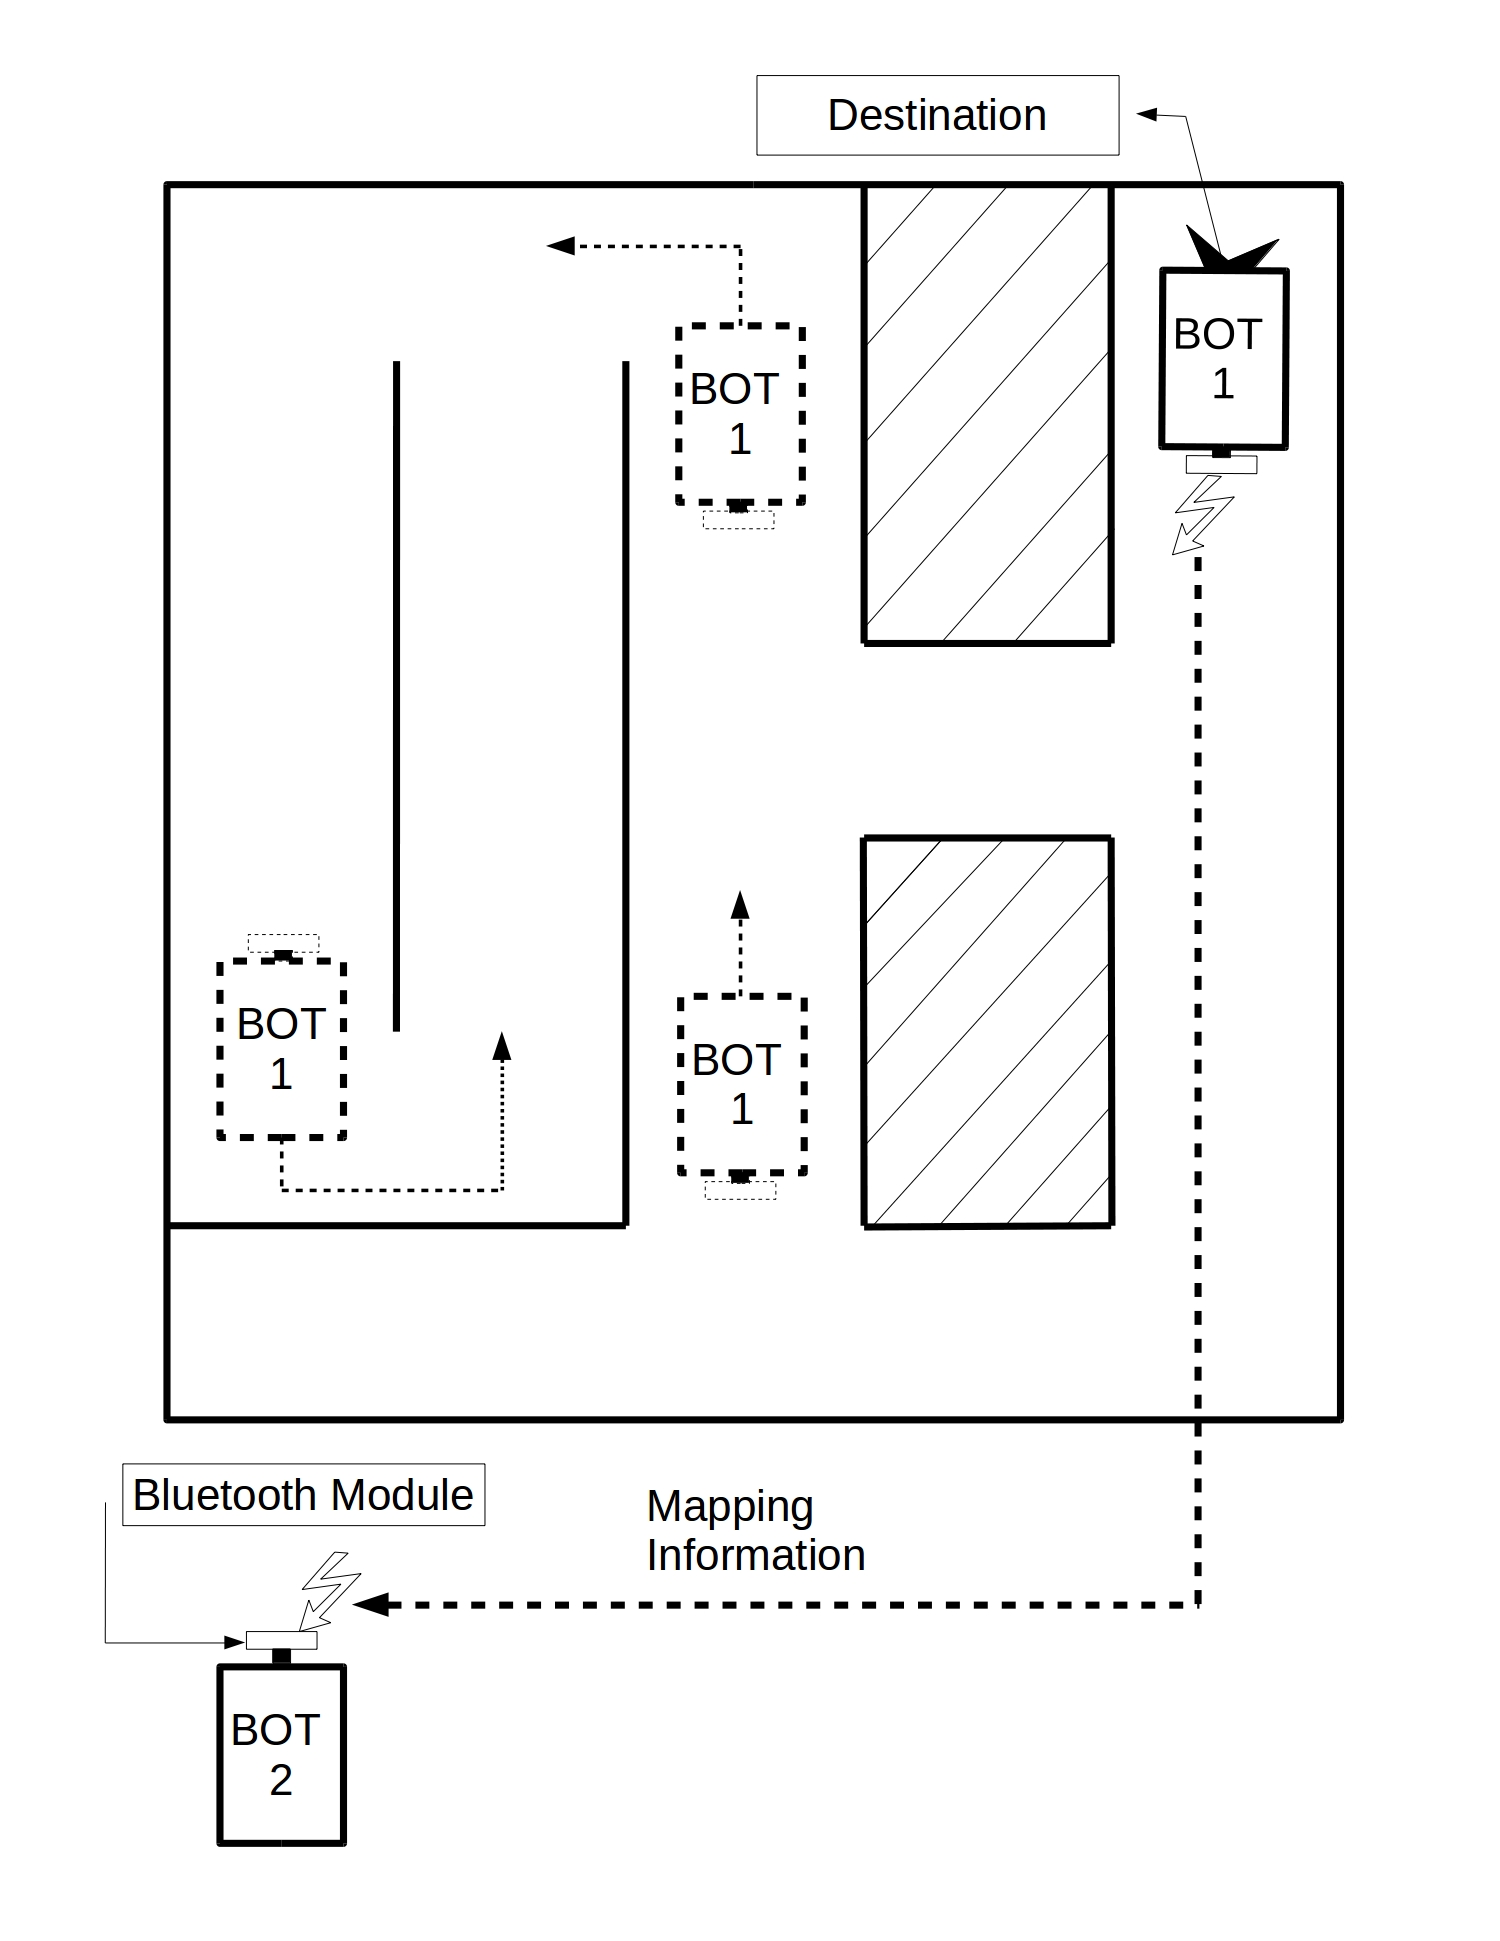
\includegraphics[scale=0.25]{systemblockdiagram_new.jpg} 
\caption{System Architecture}
\end{figure}
\justify The system contains two robotic agents. The two agents don't share the maze at the same time. First, one agent traverses the whole maze and relays the information it gathered, to the second agent via Bluetooth. The second agent will use the information provided by the first agent to solve the maze through the most optimal path. \\
The complete functional block diagram of the system is as shown below:
\begin{figure}[h]
\center
  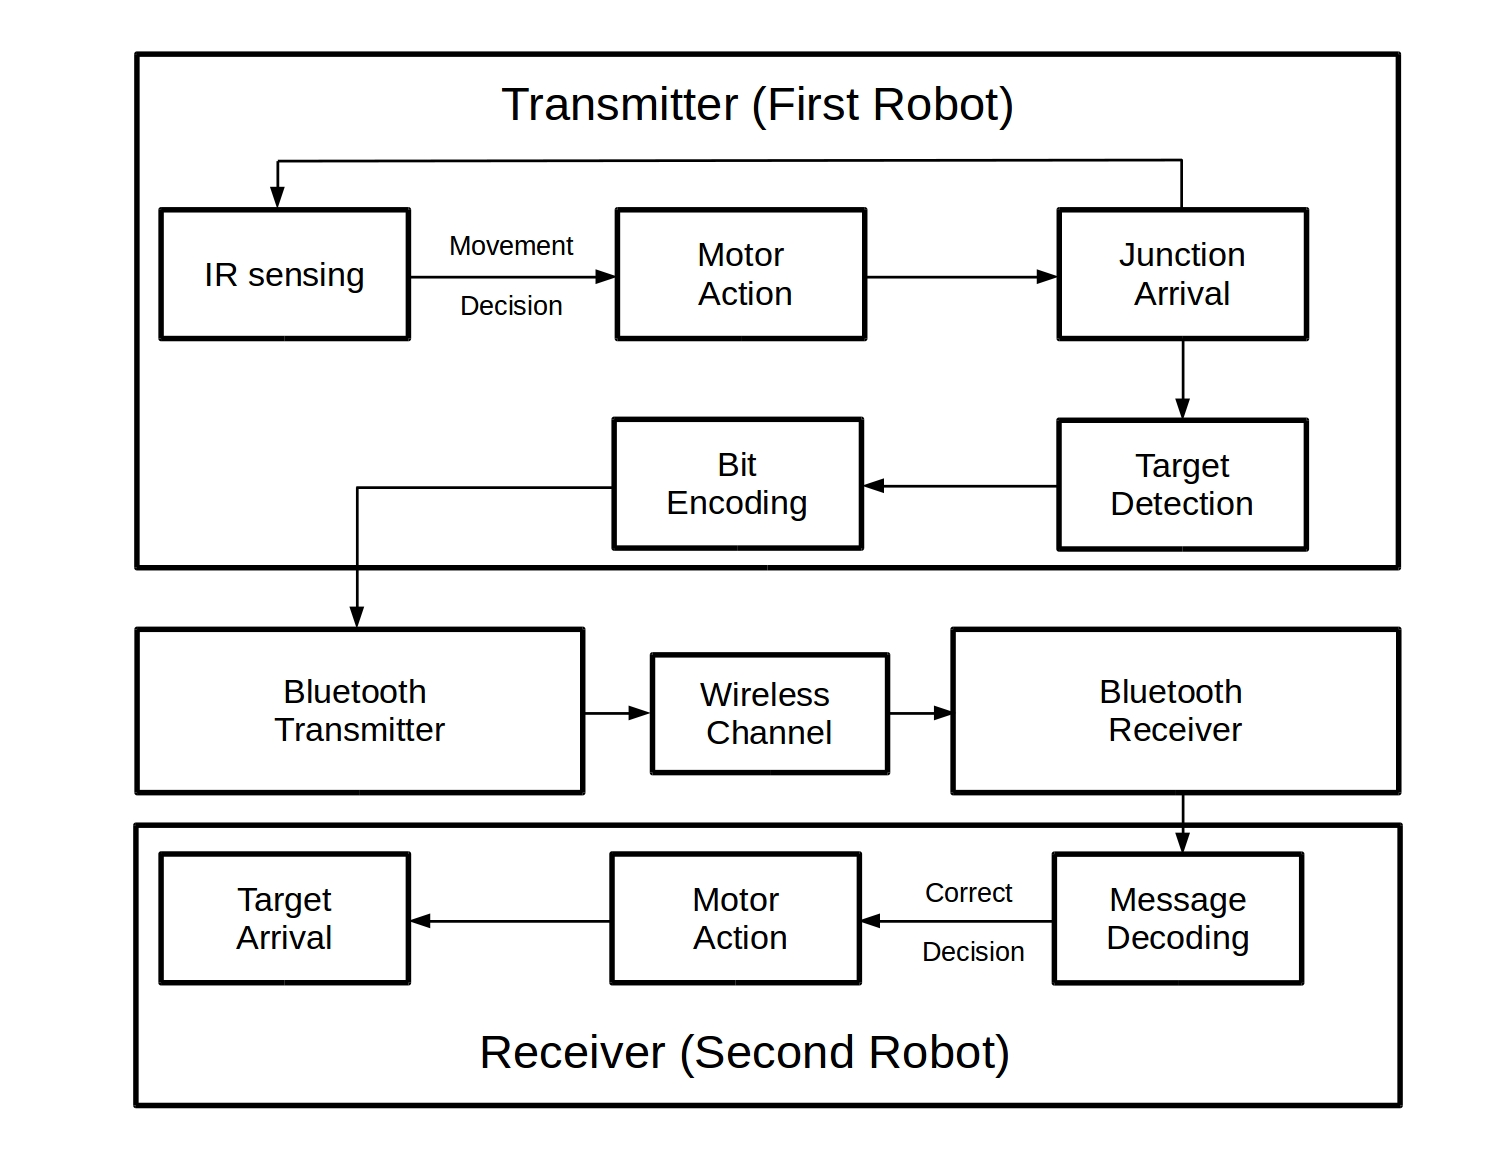
\includegraphics[scale=0.25]{funtionblock_new.jpg} 
\caption{The functional block Diagram for the system}
\end{figure}
\justify The maze solving is carried out in several steps as shown by the functional block diagram. First, the IR  sensors in the first robot detect the walls based upon which the movement decision is made. The motor action takes place according to the movement decision which is determined by the program in the microcontroller. As the motor action takes the drives the robot either left, straight or right, it reaches a junction at some point. Until the target is detected by the smoke sensor, the above process continues.\\
When the target has been detected, the shortest path information is encoded and sent to the second robot through bluetooth. Air acts as the channnel for transmission of information where noise is added during transmission. At the receiving side i.e. the second robot the information is decoded into direction information at the junction. These decisions are carried out only at the junctions which is again detected through IR sensing. The difference between the two robots is that, the second one takes the correct direction when it encounters a junction and through respective motor action, it reaches the target. 
